\section{Analyse}\label{sec:analyse}
In diesem Kapitel der Arbeit werden zunächst existierende Plattformen am Markt verglichen und darauf aufbauend Anforderungen an das Projekt formuliert.
\subsection{Vergleich mit existierenden Plattformen}\label{sec:vergleichplat}
Im folgenden Abschnitt werden ausgewählte existierende Plattformen, die im Bereich 
digital gestützte Unterrichtsmethoden angesiedelt sind, beleuchtet und anschließend 
gegenübergestellt. Eine klare Trennung zwischen kommerziell und nicht-kommerziell ist schwierig bis unmöglich, da viele Plattformen im Bereich des Freemium\footnote{Freemium ist ein Geschäftsmodell, bei dem das Basisprodukt gratis angeboten wird, während das Vollprodukt und Erweiterungen kostenpflichtig sind.} Geschäftsmodells vermarktet werden. Generell gibt es sehr viele Anbieter und Plattformen und somit ist eine Beschränkung der Auswahl unabdingbar. 
% es gibt sehr sehr viele tools, eine Beschränkung im Vergleich ist unabdingbar. 
% viele tools machen dinge verschieden. Beispiel single user prinzip (mind maps)

\paragraph{SMART Learning Suite Online}\cite{slso}
Der Anbieter SMART (Smart Technologies Corporation) ist in Deutschland vor allem für sein Angebot von interaktiven Whiteboards, welche unter dem Namen SMART Board vermarktet werden, bekannt. Ergänzend bietet SMART auch die SMART Learning Suite an, welche sowohl online als auch als lokale Installation genutzt werden kann. Positiv hervorzuheben ist, dass bei der Cloud Variante der Nutzende vorab seine Server Region festlegt. Wird hier Europa gewählt, ist anzunehmen dass europäische Richtlinien im Bezug auf Datenschutz und Speicheranforderungen berücksichtigt werden. Gespeichert werden die Daten generell auf Amazon- oder Google-Servern, wobei Smart angibt, dass in der europäischen Service Region hierbei Amazon-oder Google-Server mit Standort Deutschland genutzt werden\cite{Technologies2019}. Die SMART Learning Suite kann sowohl online als auch offline installiert werden und kostenlos getestet werden. Getestet wurde jedoch nur die online Version, da nur diese im Webbrowser läuft, welches in Hinsicht auf dieses Projekt relevant ist. \\ Das Angebot umfasst viele Funktionalitäten und unterschiedlichste Implementierungen von  interaktiven Unterrichtsmethoden, wie Quiz/Befragungen, Brainstorming, Memory, Karteikarten u.v.m. Viele Anwendungen funktionieren im Einzelanwender-Betrieb, Lehrender, Schülerinnen und Schüler nutzen das gleiche Gerät. Andere Anwendungen erfordern zusätzliche Clients, sprich Geräte wie Smartphones oder Computer, laufen also im Mehrbenutzerbetrieb. Ebenso können Lehrende Prüfungsaufgaben erstellen und diese dann Abfragen und Auswerten. Eine strikte Unterscheidung zwischen Lehrer-, Klassen-, und Studierendenansicht findet nicht statt. Ein großer Anspruch der Software ist, dass ein Lehrender ein ganzes Set an Aktivitäten für den Unterricht erstellen kann und dieses schrittweise durchlaufen wird. Es kann bspw. mit einem Test begonnen werden, anschließend erfolgt ein Folie mit einem Begriff und darauffolgend wird ein interaktive Unterrichtsmethode ausgeführt usw. 
% Sehr cool und mächtig, doof beim brainstorming, begriff steht nicht in der mitte? Sehr klein alles! Nicht lokalisiert auf Deutsch

\begin{figure}[H]
	\centering
	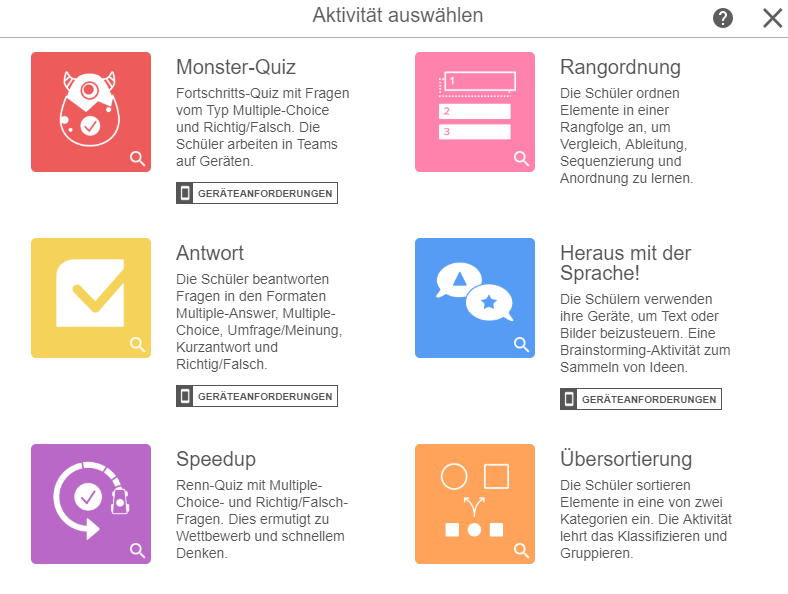
\includegraphics[width=0.8\linewidth]{bilder/screenshot_slo}
	\caption[Screenshot SMART Learning Suite Online]{Screenshot SMART Learning Suite Online:\\ Im Bild ist die Maske zur Aktivitätserstellung zu sehen. \\ Benötigen die Schüler ein Endgerät, so wird dies gekennzeichnet \cite{slso}}
	\label{fig:slso}
\end{figure}

\paragraph{ClassFlow}
Ähnlich zu SMART Learning Suite Online ist ClassFlow eine Software, welche das 
Durchführen von interaktivem Unterricht ermöglicht. Der Lehrende erstellt hierzu Sitzungen, welche ähnlich einer Präsentation durchlaufen werden. An jeder Stelle kann der Lehrende den Bildschirminhalt an die Schülerinnen und Schüler Endgeräte schicken und interaktive Unterrichtsmethoden starten, welche z.B. Umfragen, Brainstormings, Kreuzworträtsel u.v.m. sein können. Die Software läuft in der Cloud, es existiert keine Offline Variante. Für eine reine Datenspeicherung innerhalb der EU garantiert der Anbieter Promethean Limited nicht\cite{Limited2017}. Es können auch die meisten interaktiven Unterrichtsmethoden, in ClassFlow Aktivitäten genannt, im Einbenutzerbetrieb genutzt werden, d.h. die Einheit wird auf einem Computer gestartet und dort auch ausgeführt. Weitere Geräte seitens der Schülerinnen und Schüler sind dann nicht notwendig. Eine interaktive digitale Tafel ist in diesem Modus jedoch empfehlenswert. Lehrende können auch schon vorgefertigte Unterrichtseinheiten aus dem sog. Marktplatz erwerben. Es gibt kostenlose wie auch kostenpflichtige Einheiten. 

\begin{figure}[H]
	\centering
	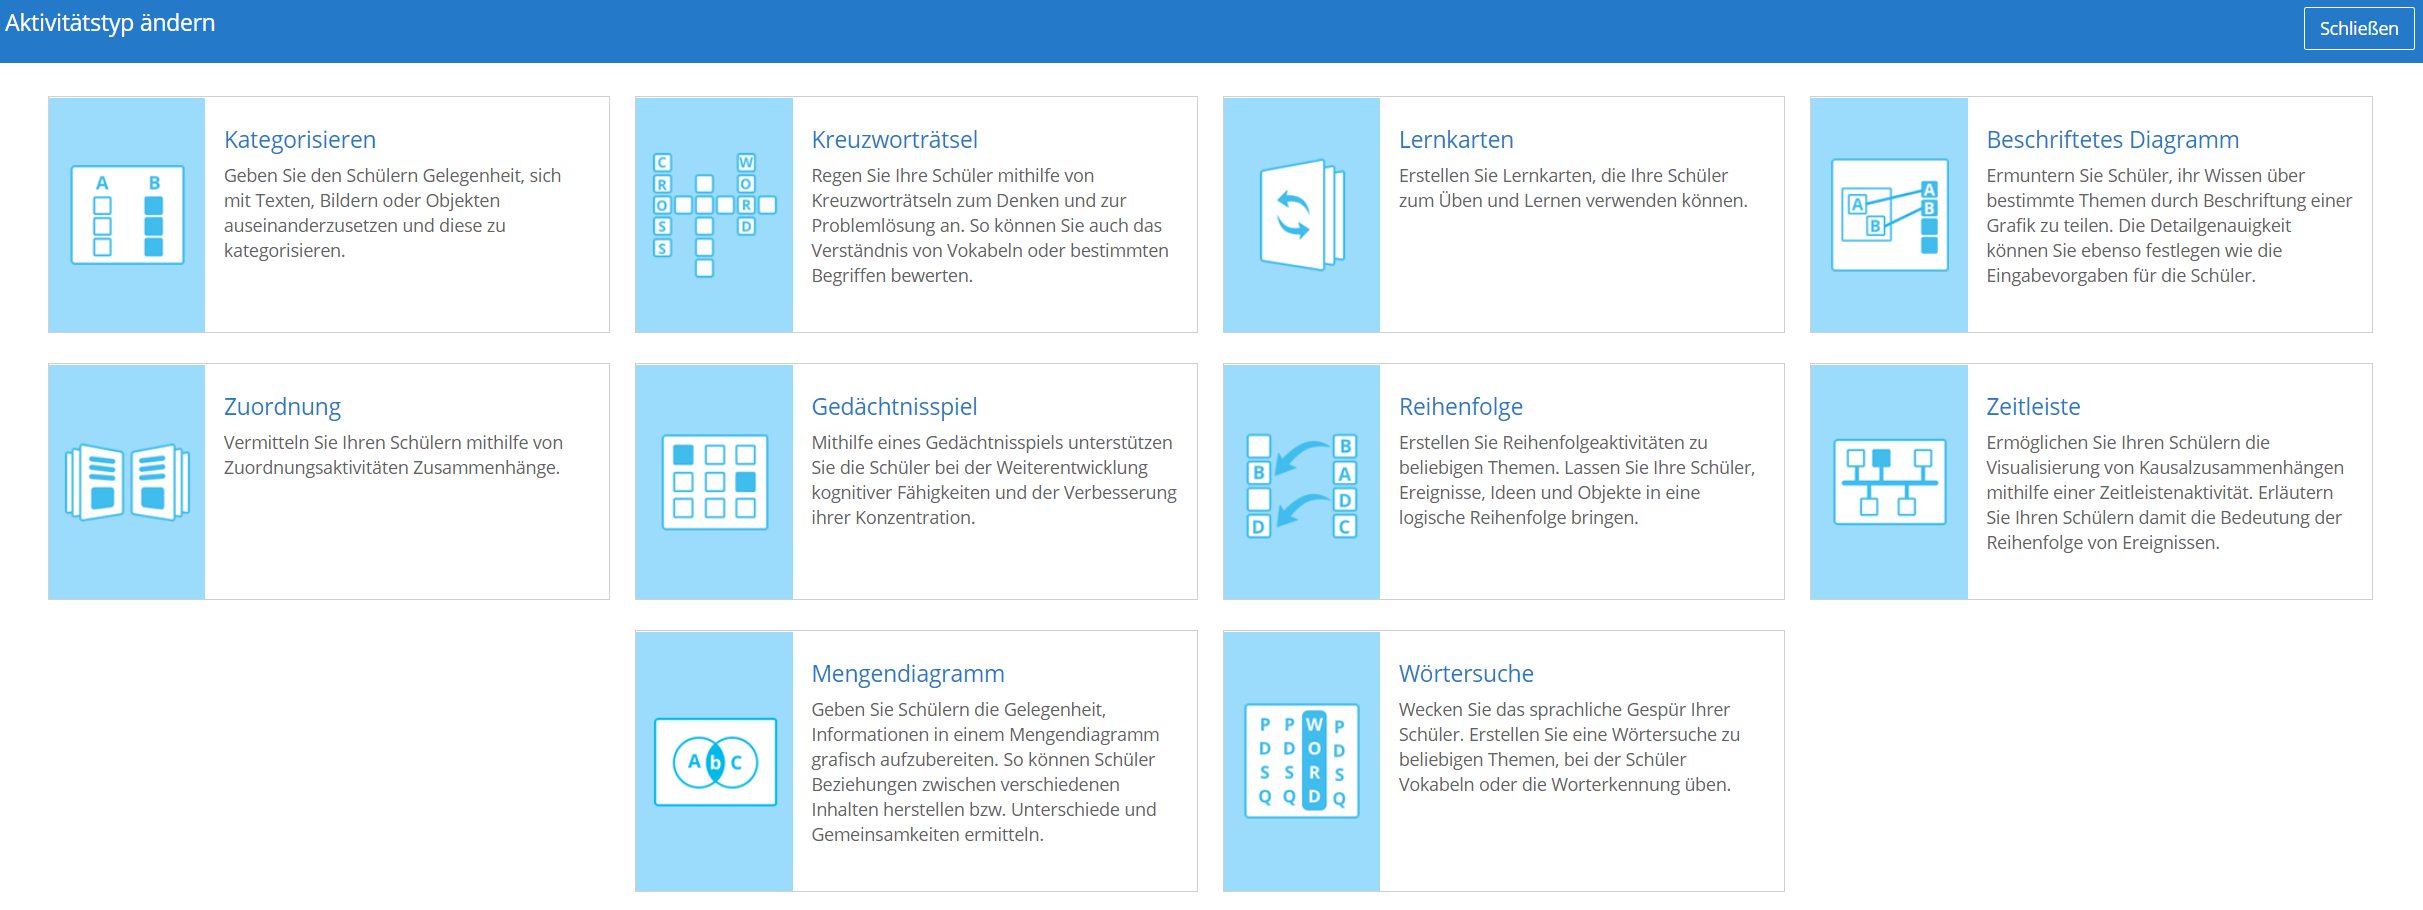
\includegraphics[width=0.8\linewidth]{bilder/screenshot_classflow}
	\caption[Screenshot ClassFlow]{Screenshot ClassFlow:\\ Aktivitäten können i.d.R. am gleichen Gerät ausgeführt sowie an Endgeräte der Schüler geschickt werden. \cite{PrometheanLimeted2019}}
	\label{fig:slso}
\end{figure}

\paragraph{Google Classroom}
Die online Software Google Classroom ist eng in die Produktpalette der Firma Google inc. eingebettet. Technisch betrachtet lässt sich Google Classroom eher mit der Software Moodle vergleichen, da eher das Ziel der Organisation einer Bildungsreinrichtung bzw. derer Kurse und Klassen verfolgt wird, obgleich das erstellen von Fragen an alle Kursteilnehmer sowie von Quiz Aufgaben möglich ist. Beim Quiz wird die hauseigene online Software Google Formulare verwendet. Bildungseinrichtungen müssen sich zunächst als solche registrieren, bevor eine Nutzung erlaubt wird. Man kann Google Classroom allerdings auch privat mit einem Google Konto nutzen, wenn explizt angegeben wird, dass die Software nicht in einer Bildungseinrichtung genutzt wird. Bildungsreinrichtungen müssen ein G Suite for Education Konto eröffnen, welches die Verwendung und Verwaltung weiterer Google Software mit sich bringt, so z.B. Google Kalender, G-Mail und weitere. Eine analoges Softwareangebot besteht auch für Unternehme namens G Suite. Der Google eigene Cloudspeicherdienst Google Drive ist angebunden und somit werden z.B. erstellte Quizze dort abgespeichert.  Beim Speichern der Daten kann von nicht EU-zentralen Google eigenen Cloud-Servern ausgegangen werden. 

\paragraph{Sonstige}
Neben den o.g. größeren Anbietern existieren viele kleinere Online Angebote, welche sich meist auf die Bereitstellung einer Dienstleistung bzw. Ausführung einer interaktiven Unterrichtsmethode beschränke, hierbei jedoch oftmals auch interessante Ansätze zu finden sind. Gerade wenn Dozierende unkompliziert eine bestimmte interaktive Unterrichtsmehthode im Unterricht einsetzen möchte, bietet es sich an auf einen kleineren Anbieter zurückzugreifen. Zu nennen wäre hier z.B. die Software \textbf{Plickers}, welche das Prinzip bring-your-own-device etwas abändert. Die Schülerinnen und Schüler benötigen hier lediglich Papier auf dem spezielle QR-Codes abgebildet sind. Bei Fragestellungen wird das Papier nach oben gehalten und je nachdem welche Seite des Papiers (und somit auch des QR-Codes) nach oben zeigt, wird entschieden ob für Antwort A, B, C oder D plädiert wird. Eine Kamera vom Smartphone oder Tablet des Dozierenden erkennt dies und kann somit die Daten auswerten. Ähnlich verfährt die Anwendung \textbf{Poll Everywhere}, hier ist allerdings ein Endgerät pro Schülerin bzw. Schüler notwending. Wer nur teilnimmt muss jedoch keine Applikation installieren, hier reicht ein spezieller Link der in einem Webbrowser aufgerufen wird.  
% Freemium modell auch, hier geben die Leute via app die antwort
% geteiltes Client prinzip (Presenter and teacher view)
% Gezielt für Umfragen, nicht quiz
% wohl kostenlos
\subsubsection{Gegenüberstellung}\label{sec:gegenstellung}
Nach der Präsentation der ausgewählten Angebote in Abschnitt \ref{sec:vergleichplat} werden diese in folgenden Hauptkriterien miteinander verglichen:
\begin{enumerate}
	\item \textbf{Serverstandort}: Werden die Server des Anbieters innerhalb der Europäischen Union betrieben, sodass datenschutzrechtliche Regelungen dieser Anwendungen finden?
	\item \textbf{Online Nutzung}: Ist die Nutzung über das Internet möglich? 
	\item \textbf{Offline Nutzung}: Ist die Nutzung offline über das Intranet möglich? 
	\item \textbf{Betriebsart E/M}: Ist die Nutzung im Einzelbenutzerbetrieb und/oder im Mehrbenutzerbetrieb möglich? Ersteres bedeute, dass eventuell mehrere Nutzer die Software ggf. an einem Computer verwenden können, eine Interaktion über mehrere angebundene Clients ist nicht möglich. Im Mehrbenutzerbetrieb können sich können sich Nutzende über Clients mit der Software verbinden und gemeinsam interaktiv werden.
	\item \textbf{Betriebsmodus (Single/Set)}: Können mehrere Unterrichtsmethoden als Set angelegt werden, welches später sukzessiv durchlaufen wird oder können nur einzeln angelegte Unterrichtsmethoden nach und nach manuell gestartet werden? (Single)
	\item \textbf{Clients}: Gibt es unterschiedliche  Arten von Clients für Lehrende, Teilnehmende und spezielle, die nur zur Anzeige gedacht sind?
	\item \textbf{Registrierung}: Ist für die Nutzung eine Registrierung für Lehrende notwendig? Ebenso für Schülerinnen und Schüler?
	\item \textbf{Unterstützte Unterrichtsmethoden}: Welche lassen sich nutzen? Bei mehr als zwei wird hier die reine Zahl genannt.  
\end{enumerate}

% \usepackage{booktabs}
\begin{table}[h!]
	\caption{Tabellarischer Vergleich existierender Plattformen}
	\label{tab:vergplatt}
	\resizebox{\textwidth}{!}{%
	\begin{tabular}{@{}|l|c|c|c|c|c|@{}}
		\toprule
		\textbf{Produkt}    & \textbf{SMART LSO}          & \textbf{ClassFlow}           & \textbf{Google Classroom}    & \textbf{Plickers}            & \textbf{Poll Everywhere}          \\ \midrule
		Serverstandort EU   & \cellcolor[HTML]{32CB00}Ja* & \cellcolor[HTML]{FE0000}Nein & \cellcolor[HTML]{FE0000}Nein & \cellcolor[HTML]{FE0000}Nein & \cellcolor[HTML]{FFCC67}Unbekannt \\ \midrule
		Online Nutztung     & \cellcolor[HTML]{32CB00}Ja  & \cellcolor[HTML]{32CB00}Ja   & \cellcolor[HTML]{32CB00}Ja   & \cellcolor[HTML]{32CB00}Ja   & \cellcolor[HTML]{32CB00}Ja        \\ \midrule
		Offline Nutzung     & \cellcolor[HTML]{32CB00}Ja  & \cellcolor[HTML]{FE0000}Nein & \cellcolor[HTML]{FE0000}Nein & \cellcolor[HTML]{FE0000}Nein & \cellcolor[HTML]{FE0000}Nein      \\ \midrule
		Betriebsmodus       & Single/Set                  & Single/Set                   & Single                       & Single                       & Single                           \\ \midrule
		Clients             & 2 (Lehrer/Schüler)          & 2 (Lehrer/Schüler)           & 2 (Lehrer/Schüler)           & 2 (Lehrer/Schüler)**         & 2 (Lehrer/Schüler)                \\ \midrule
		Registrierung       & Ja/Nein                     & Ja/Ja                        & Ja/Ja                        & Ja/Nein                      & Ja/Nein                           \\ \midrule
		Unterrichtsmethoden & 12                          & 10                           & Frage/Quiz                   & Quiz                         & Umfragen                          \\ \bottomrule
	\end{tabular}
}
\footnotesize {
	* Option ist innerhalb der Software wählbar. \\
	** Der 'Client' für die Schülerinnen und Schüler stellt in diesem Fall Papier mit aufgedruckten QR Codes da.
}

\end{table}

Aus der Tabelle lässt sich erschließen, dass SMART Learning Suite Online und ClassFlow einen ähnlichen Ansatz nutzen und in unmittelbarer Konkurrenz 
zueinander stehen. Beide bieten viele Arten von interaktiven Unterrichtsmethoden an und sehen den Betrieb als Software vor, die eine gesamte Unterrichtseinheit als solche unterstützt und in ihr eine leitende Funktion einnimmt. Es können einzelne Methoden gestartet werden, doch die hauptsächliche Stärke findet sich in dem Erstellen von Sets, welche dass iterative Abarbeiten von Folien und interaktiven Unterrichtsmethoden vorsieht. Die zwei größten Vorteil von SMART Learning Suite Online sind einerseits der verfügbare Einsatz von Offline Applikationen, welche allerdings installiert werden müssen, was die genannten Nachteile aus Sektion \ref{sec:vorundnachteileweb} mit sich bringt, und dem Serverstandort innerhalb der EU, welcher explizit festgelegt werden kann. ClassFlow bietet dafür noch mehr Interaktion auch außerhalb der Ausführung von interaktiven Unterrichtsmethoden, da der Lehrende z.B. jederzeit das aktuelle Tafelbild an die angeschlossenen Clients der Schülerinnen und Schüler schicken kann. Dabei kann auch zwischen Gruppen unterschieden werden. Wird das Tafelbild von einem Client verändert, kann der Lehrende dies akzeptieren und z.B. als neue Grundlage für den weiteren Unterricht verwenden. Schülerinnen und Schüler können die SMART Learning Suite Online auch anonym nutzen, während dies bei ClassFlow nicht möglich ist, wobei dieses vorgehen ohnehin der Betriebsart hinderlich sein könnte. Die Anbieter Plickers und Pull Everywhere sind fokussierter auf das Anbieten einer interaktiven Unterrichtsmethode. Beide Angebote können auch gut von Unternehmen und anderen Nutzenden während Präsentationen und Vorträgen genutzt werden, die eindeutige Nutzung innerhalb einer Bildungseinrichtung ist nicht gegeben aber auch bewusst nicht gewünscht. Da nur eine Unterrichtsmethode existiert, ist kein Set-Betrieb möglich. Alle Anbieter haben gemein, dass sie keinen speziellen Client oder sonstige Lösung für reine Präsentationsgeräte wie Projektoren oder andere Großbild-Anzeigen anbieten. Dieser Punkt soll in der zu entwickelnden Software gelöst werden. Keine der genannten Anbieter lässt den Betrieb als im Intranet laufende Webanwendung zu, dies erschwert den Zugang für minder technisch ausgestattet Bildungseinrichtungen. Gehobener Datenschutz, bei dem die Daten gar nicht erst das Intranet verlassen, ist ebenfalls nicht gegeben. \\ \\
Der Vergleich zeigt folgende wünschenswerte Eigenschaften für die im Rahmen dieses Projektes zu implementierende Software auf:
\begin{itemize}
	\item Ein Betrieb unabhängig vom Internet ist wünschenswert um den Einsatz in Einrichtungen ohne gut ausgebaute oder gar nicht vorhandene Internetanbindung zu ermöglichen. Hierzu sollte wenn möglich autark ein Intranet durch einen WLAN-Zugangspunkt ermöglicht werden, welcher selbstständig ein Netzwerk aufbaut und Clients die Verbindung ermöglicht. Ein Betrieb im Intranet würde ggf. das Aufkommen datenschutzrechtliche Fragen deutlich eindämmen.
	\item Ein zusätzlicher Präsenter Client, welche unabhängig und bei Bedarf auf einer anderen Maschine ausgeführt wird, bringt mehr Flexibilität für den Dozierenden. So kann der Lehrende bspw. sein Smartphone als Kontrollclient nutzen und den im Klassenraum installierten Rechner, welcher an ein Projektor oder interaktive Tafel angeschlossenen ist zur reinen Anzeige der relevanten Inhalte nutzen. Diese Anzeige kann zusätzlich auf die visuellen Ansprüche eine Großbildanzeige optimiert sein, sodass ein Betrachten auch aus weiterer Entfernung problemlos möglich ist. Je nach Situation können Server und Clients aber auch einfach auf derselben Maschine ausgeführt werden. 
	\item Die Installation und Inbetriebnahme der Serversoftware sollte so einfach wie möglich gestaltet werden, um auch weniger technisch versierten Dozierenden die Nutzung zu vereinfachen. Deshalb sollte auch eine Installation, welche tiefer ins System eingreift, möglichst vermieden werden. Ein rein im Internet angebotener Dienst muss diesen Teil natürlich nicht berücksichtigen und kann die technische Wartung selbst übernehmen.
	\item Das Anbieten mehrere interaktiver Unterrichtsmethoden innerhalb der Software ist wünschenswert, um die Nutzung und Inbetriebnahme attraktiver zu machen und die Fragmentierung der Inanspruchnahme mehrere Anbieter seitens der Nutzenden einzudämmen. 
\end{itemize}





%Nicht Funktional:
%- Erreichbarkeit: Offline im Intranet
%- Wartbarkeit: Anzeige von Fehlern
%- Nutzung von freier Software
%- Performanz: Ohne nenns. verzögerung
%- Portierbarkeit: OS Unabhängig
%- Usability: egal welches device
%- Sicherheit: PW speichern, HTTPS

\subsection{Systembeschreibung}\label{sec:sysbeschreib}
Aus Gründen der Lesbarkeit wurde im folgenden Abschnitt die männliche Form gewählt, nichtsdestoweniger beziehen sich die Angaben auf Angehörige beider Geschlechter. \\ 

Die Software soll als Web Server-Applikation implementiert sein. Diese soll skalierbar sein, d.h. ein Betrieb rein im Intranet ohne großen Installationsaufwand soll möglich sein als auch der Betrieb auf einem entfernten, via Intranet oder Internet angebundenen Server. Die Software soll auch ohne aktive Internetanbindung im Intranet (resp. LAN) nutzbar sein.
Über zwei Web-Client Lösungen kann mit dem Server interagiert werden, eine für Lehrende, eine für Schüler. Ein dritter Client, welche unabhängig fungiert, ist für den Einsatz auf Anzeigegeräten wie Projektoren und sonstigen Großbild-Anzeigen gedacht.  

Über ein Backend Zugang können Administratoren und Dozierende den Server verwalten sowie erstmalig initialisieren. Neue Dozierende können einen Benutzeraccount anlegen, welcher von Administratoren freigeschaltet werden muss. Alternativ können Administratoren neue Benutzerkonten anlegen. Dozierende ist es möglich Lehreinheiten (auch Set genannt) zu erstellen, diese zu starten sowie zu beenden. Während einer aktiven Lehreinheit, ist es Dozierenden möglich, diese zu leiten. (Fortschritt, Verbundene Schüler/Studenten verwalten, Speichern, je nach Typ der Lehreinheit.) Eine Lehreinheit besitzt eine oder mehrere interaktive Unterrichtsmethodiken softwareseitig umgesetzt. Als erste Umsetzung erfolgt in diesem Projekt die Implementierung eines Brainstorming und Quiz. Der parallele Betrieb von mehreren, unabhängig am System authentifizierten Lehrenden, welche Lehreinheiten starten und zu denen sich Schülerinnen und Schülern einschreiben, soll möglich sein.

Ein Präsenter Client zeigt die zur Laufzeit einer aktiven Lehreinheit und seiner interaktiven Unterrichtsmethode relevanten Informationen an. Dieser ist zur Anzeige auf einem Großflächenanzeigegerät ausgelegt (Projektor, Fernseher, Smart Board). Es soll problemlos möglich sein, mehrere Präsenter Clients anzukoppeln. \\ 

Schüler/Studenten geben einen frei wählbaren Namen an. Ein Benutzerregistrierung ist nicht notwendig. Sie können anschließend aktiven Lehreinheiten beitreten und nach dem Start an deren interaktiven Unterrichtsmethoden partizipieren. \\

Eine detaillierte Aufführung der Anforderungen und Eigenschaften dieses Projekts erfolgt in den nachfolgenden Abschnitten. 

\subsection{Zielgruppe}\label{sec:zielgruppe}
Das Software-Projekt soll sich in erster Linie an Bildungseinrichtungen jeglicher Art und deren Dozierenden richten, welche eine lokal ausgeführte Softwarelösung für das Durchführen von interaktiven Unterrichtsmethoden bevorzugen. Darüber hinaus auch an jegliche, die digital gestützte interaktive Lern- und kompetitive Kleinstspiele nutzen möchten. Dabei ist eine flexible Skalierbarkeit des Servers gegeben (siehe Abschnitt \ref{sec:anforderung}). Des weiteren ist das Software-Projekt attraktiv für die Open-Source Community, welche das Projekt weiter ausbauen kann sowie neue Typen von Lehreinheiten (interaktive Unterrichtsmethode softwareseitig umgesetzt / 'Spiel'-Art) hinzufügen kann.
\subsection{Abgrenzung}\label{sec:abgrenz}
Der Prototyp des Softwareprojekts (interne Bezeichnung Node ICT \footnote{Node ICT steht für Node.js interactive course teaching. Das Node.js Server Framework bildet den Grundstein des Softwareprojekts}) soll das Anlegen und Ausführen von Lehreinheiten mit zunächst einer interaktiven Unterrichtsmethode ermöglichen. Der Prototyp wird auf dem lokalen Host getestet (Server und Client auf derselbe Maschine ausgeführt) sowie im Intranet (LAN, Server und Clients auf unterschiedlichen Maschinen ausgeführt). Eine verschlüsselte Kommunikation zwischen Server und Client ist erwünscht, wird jedoch nicht im Prototyp implementiert. Eine Nutzung über öffentlicher IP-Adresse oder Domain im Internet ist prinzipiell möglich, wird jedoch nicht getestet. Ebenso wird bei dem Prototyp vermindert Augenmerk auf das Design der Client Anwendungen gelegt, worunter die Usability jedoch nicht leiden soll. Das Design wird leicht anpassbar sein. Wie in Abschnitt \ref{sec:sysbeschreib} erwähnt, wird sich auf das Implementieren von zwei interaktiven Unterrichtsmethoden beschränkt, der Prototyp wird aber das Umsetzen und Hinzufügen weitere Unterrichtsmethoden ermöglichen, da prinzipielle nur die Logik der neuen Unterrichtsmethode geschrieben werden muss. Eine Wiederverwendbarkeit von grundlegender Funktionalität (z.B. Anbindung an Datenbank, Management verbundener Clients etc.) wird bereitgestellt. Zunächst wird pro Lehreinheit (Set) nur eine interaktive Unterrichtsmethode zugewiesen werden können.  
\subsection{Systemanforderungen}\label{sec:anforderung}
Aufbauend auf das Analysekapitel dieser Arbeit (Abschnitt \ref{sec:analyse} ff.) sowie dem Abschnitten \ref{sec:digianschulen} und \ref{sec:datenschutz} lassen sich funktionale und nicht-funktionale Anforderungen an das System ausformulieren, welche in den folgenden zwei Abschnitten gelistet werden.

% Verschlüsselung HTTPS
% Siehe BA von Michelle
\subsubsection{Nicht Funktional}\label{sec:nichtfunc}
Die Erstellung der nicht funktionalen Anforderungen an das System wurde aufbauend auf 
dem Vergleich existierender Plattformen aus Abschnitt \ref{sec:vorundnachteileweb} angefertigt,
wobei noch weitere für das Projekt als wichtig erachtete Aspekte mit eingeflossen sind. 
% Please add the following required packages to your document preamble:
% \usepackage{booktabs}
% \usepackage[table,xcdraw]{xcolor}
% If you use beamer only pass "xcolor=table" option, i.e. \documentclass[xcolor=table]{beamer}
\begin{table}[h!]
	\caption{Nicht Funktionale Anforderungen an die Projektsoftware}
	\label{tab:nichtfunkanf}

\begin{tabular}{@{}cll@{}}
	\toprule
	\rowcolor[HTML]{FFFFFF} 
	\textbf{ID} & \multicolumn{1}{c}{\cellcolor[HTML]{FFFFFF}\textbf{Name}}                    & \multicolumn{1}{c}{\cellcolor[HTML]{FFFFFF}\textbf{Beschreibung}}                                                                                                             \\ \midrule
	\rowcolor[HTML]{FFFFFF} 
	NFA01       & Erreichbarkeit                                                               & \begin{tabular}[c]{@{}l@{}}Das System soll auch ohne jeglichen Internetzugang\\ im Intranet betrieben werden können\end{tabular}                                              \\
	\rowcolor[HTML]{EFEFEF} 
	NFA02       & Wartbarkeit                                                                  & \begin{tabular}[c]{@{}l@{}}Der Code der Software soll verständlich und\\ einfach zu warten und erweitern sein\end{tabular}                                                    \\
	\rowcolor[HTML]{FFFFFF} 
	NFA03       & \begin{tabular}[c]{@{}l@{}}Nutzung von\\ Open-Source\\ Software\end{tabular} & \begin{tabular}[c]{@{}l@{}}Die Nutzung von Open-Source Modulen und\\ Frameworks ist zu bevorzugen\end{tabular}                                                                \\
	\rowcolor[HTML]{EFEFEF} 
	NFA04       & Performanz                                                                   & \begin{tabular}[c]{@{}l@{}}Das System soll ohne nennenswerte Verzögerung\\ auf Eingaben reagieren\end{tabular}                                                                \\
	\rowcolor[HTML]{FFFFFF} 
	NFA05       & Portierbarkeit                                                               & \begin{tabular}[c]{@{}l@{}}Der Betrieb unter unterschiedlichen Betriebssystemen\\ soll möglich sein\end{tabular}                                                              \\
	\rowcolor[HTML]{EFEFEF} 
	NFA06       & Usability                                                                    & \begin{tabular}[c]{@{}l@{}}Die Anzeige und die damit einhergehende Usability\\ soll auf das verwendete Gerät angepasst sein\end{tabular}                                      \\
	\rowcolor[HTML]{FFFFFF} 
	NFA07       & Sicherheit                                                                   & \begin{tabular}[c]{@{}l@{}}Die Verbindung zwischen Client und Server soll\\ verschlüsselt sein. Daten wie Passwörter sollen ver-\\ schlüsselt gespeichert werden\end{tabular}
\end{tabular}


\end{table}
\newpage
\subsubsection{Funktional}\label{sec:anffunc}
% Anhang?
% Siehe ARbeit Michelle, selbst formulieren einfach?
% Funktional:
%- Datenbankanbindung
%- Erstellung der Datenbank
%- REaktion GET Requests
%- Reaktion POST Request
%- Login System Sessions
%- MVC Pattern
%- Socket Verbindungen
%- Einfach Client Konnektivität: QR
%- 3 Client Prinzip
%- Ausführen von Unterrichtsmethoden

Aus Gründen der Übersicht wurden die Funktionale Anforderungen in den Anhang dieser Ausarbeitung verschoben. Diese wurden aufbauend auf den Erkenntnissen des Vergleiches existierender Plattformen aus Abschnitt \ref{sec:vorundnachteileweb} gebildet und ausformuliert. Hierbei wurde auch der Implementierungsstatus mit vermerkt, welcher chronologisch erst nach \textbf{Kapitel \ref{sec:implementierung}}, der eigentlichen Implementierung, vorgenommen wurde. 
\subsection{Technische Anforderungen}\label{sec:techanford}
In diesem Abschnitt werden die technischen Anforderungen an die Hardware erläutert, welche einen reibungslosen Betriebsablauf gewährleisten sollen. Es wird hierbei zwischen Server und Client Anforderungen unterschieden obgleich Server und Client auch auf der selben Maschine ausgeführt werden können. 
\subsubsection{Server}\label{sec:servertech}
Die Server Software soll so umgesetzt werden, dass sie auch auf leistungsschwächerer Hardware problemlos mehrere Benutzer gleichzeitig ohne signifikante Performanceeinbuße bedienen kann. Die Hardwarespezifikationen eines Raspberry Pi (Version 3B) Einplantinencomputer (Querverweis zu Abschnitt \ref{sec:einfuhrung}) soll hierbei als Mindestanforderung definiert sein. Durch die Nutzung des Serverwebframeworks 'Node.js' als Grundgerüst der Software, ist ein plattformunabhängiger Betrieb gewährleistet. Der Server soll rein im Intranet lauffähig sein und keine online Abhängigkeiten besitzen. Daher soll technisch keine (Breitband)Internetanbindung für den Betrieb notwendig sein. Es soll ebenso möglich sein den Server 'headless', d.h. ohne angeschlossene Peripheriegeräte wie Tastatur, Maus und Bildschirm zu betreiben. Die Initialisierung der Software kann hierbei durch ein Startskript oder beispielsweise über einen SSH\footnote{Mittels SSH (Secure Shell) kann eine verschlüsselte Verbindung zur Kommandozeile (Shell) auf einem Server hergestellt werden} Zugang erfolgen.
\subsubsection{Client}\label{sec:clienttech}
Der im Rahmen dieses Projekts zu entwickelnde Client Software kann wie in Abschnitt \ref{sec:sysbeschreib} erläutert, in drei Parts eingeteilt werden. Die Verwaltung im Backendbereichs der Server Software soll eine besonders niedrige Hardwareanforderung aufweisen, da hier gänzlich auf den Einsatz von JavaScript verzichtet werden wird. Dies soll eine Server-Verwaltung auch bei deaktiviertem JavaScript gewährleisten. Die restlichen Software Module sollen in jedem modernen Webbrowser auf jedem Endgerät lauffähig sein. Der Einsatz von JavaScript ist hier unverzichtbar. Eine Kompatibilitätsabdeckung von 95\% zur ECMAScript 6 (ECMAScript 2015) Spezifikation sollte vom verwendeten Webbrowser gegeben sein. Diese Anforderung erfüllen jedoch alle modernen Webbrowser (Stand 2019)\cite{ECMAScri7:online}. 
